\documentclass[12pt]{report}
\usepackage[
  final
 ,raggedbottom
%,tocbold        % uncomment to enable bold chapter titles in the ToC
                 %
                 % the style guidelines state that page numbers in the
                 % ToC should not be bold, but leave it up to the author
                 % and specific department guidelines as to how the
                 % chapter (or other section) titles should be typeset.
]{USCthesis}

% guidelines for manuscript formatting: https://graduateschool.usc.edu/wp-content/uploads/2020/11/Manuscript_Formatting_and_Documentation_Styles.pdf

%% our customizations %%%%%%%%%%%%%%%%%%%%%%%%%%%%%%%%%%%%%%%%%%%%%%%%%%
\usepackage[export]{adjustbox} % for frame option in \includegraphics
\usepackage{amsmath}
\usepackage{amssymb}
\usepackage{mathtools}
\usepackage{array}
\newcolumntype{C}[1]{>{\centering\arraybackslash}p{#1}}
\newcolumntype{B}[1]{>{\centering\arraybackslash}m{#1}}
\usepackage[utf8]{inputenc} % load inputenc before csquotes % With pdfLaTeX
\usepackage[english]{babel}
\usepackage{longtable}
\usepackage{indentfirst}
\setlength{\parindent}{0.5in}
% \usepackage[
%   backend     = biber,
%   doi         = true,
%   hyperref    = true,
%   maxbibnames = 99,
%   sortlocale  = en_US,
%   style       = numeric,
% ]{biblatex}
\usepackage[
  authordate,
  backend=biber,
  autocite=inline,
  giveninits=true
]{biblatex-chicago}

\usepackage{booktabs}
\usepackage{color, colortbl}
\usepackage{csquotes}
\usepackage{efbox}
\usepackage{enumitem}
\usepackage[shortcuts]{extdash} % use `\-/' to hyphenate words/phrases that have a dash in them
% \usepackage[tt=false]{libertine} % libertine's \ttfamily isn't that great
\usepackage{newtxtext,newtxmath} % With pdfLaTeX
% \usepackage{fontspec}
% \setmainfont{Times New Roman}
\usepackage[T1]{fontenc} % load fonts before fontenc
\usepackage[symbol]{footmisc}
\usepackage[
  showframe = false,% draw a border around textwidth
  pass      = true, % force 8.5"x11" pagesize
]{geometry}
\usepackage{graphicx}
%\usepackage[notquote]{hanging} % enables negative indents in paragraphs
\usepackage{hyphenat}
\usepackage{ifthen}
\usepackage{lipsum}
\usepackage{multirow}
\usepackage{parnotes}
% \usepackage{pdflscape} % rotate some pages in an {landscape} environment
\usepackage{lscape} % rotate page contents, but keep PDF page displayed in portrait
\usepackage{pifont}
\usepackage{ragged2e}
\usepackage{seqsplit}
\usepackage{siunitx}
\usepackage{subcaption}
\usepackage{tabularx}
\usepackage{xcolor}
\usepackage{xspace}
\usepackage{url}
\usepackage{float} % ADDED BY JEFF ROZELLE
\usepackage{threeparttable}
\usepackage{dcolumn}
% \usepackage{caption}

% \usepackage[
%   breaklinks    = false,
%   colorlinks    = false,
%   hypertexnames = false,
%   pdfpagelabels = false,
%   citecolor     = {blue!80!black},
%   linkcolor     = {blue!80!black},
%   urlcolor      = {blue!80!black}
% ]{hyperref} % load hyperref as the last package

% pkg: biblatex
\setlength\bibitemsep{0.5\baselineskip}                 % add a line between entries
\AtEveryBibitem{
  \iffieldundef{doi}{}{\clearfield{url}}
  \clearfield{note}
  \clearfield{urldate}
}

% \addbibresource{references.bib}
% \addbibresource{biblatex-references.bib}
\addbibresource{betterbiblatex-references.bib}

\DeclareSourcemap{
  \maps[datatype=bibtex]{
    \map{
      \step[fieldset=urldate, null]
      \step[fieldset=note, null]
    }
  }
}

% pkg: siunitx
% some guidelines https://physics.nist.gov/cuu/Units/checklist.html
\sisetup{
  tight-spacing  = true
  ,detect-family = true
  ,detect-mode   = true
  ,binary-units  = true    % support for MB, GB, etc.
  ,range-units   = single  % "3% to 5%" -> "3 to 5%"
  ,range-phrase  = --      % "3 to 5%"  -> "3--5%"
}

% pkg: babel, hyperref
% \addto\extrasenglish{%
%   \renewcommand{\chapterautorefname}{Chapter}
%   \renewcommand{\sectionautorefname}{Section}
%   \renewcommand{\subsectionautorefname}{Section}
%   \renewcommand{\subsubsectionautorefname}{Section}
% }

% pkg: url
\renewcommand{\UrlFont}{\footnotesize\tt}

% our custom commands
% \renewcommand{\ttdefault}{cmtt} % leave default teletype unless needed

% \newcommand{\appchapter}[1]{\chapter{Appendix \thechapter: #1}}
\newcommand{\appchapter}[1]{\chapter{#1}}

%%% draft mode / toggle commands %%%
\usepackage{etoolbox}
\newtoggle{draft}
\settoggle{draft}{true} % change toggle for draft or final versions

\iftoggle{draft}{
  % if 'draft' toggle is true
  \overfullrule=10pt                       % highlight overfull hboxes
}{
  % if 'draft' toggle is false
  \PassOptionsToPackage{final}{showlabels} % hide labels on figures, etc
}

% if you're including existing papers into your thesis, it helps to put
% content behind a toggle (or conditional) so you only have to maintain
% and keep consistency on one copy. see "introduction.tex".
\newtoggle{thesis}
\settoggle{thesis}{false}
% \proposaltrue
% \newtoggle{proposal} %!!! Jeff
% \settoggle{proposal}{true}

% \usepackage[inline]{showlabels} # labels in blue!
% \renewcommand{\showlabelfont}{\sffamily \color{blue}}
% \renewcommand{\showlabelsetlabel}[1]{\efbox{\showlabelfont #1}}
%%%%%%%%%%%%%%%%%%%%%%%%%%%%%%%%%%%%%%%%%%%%%%%%%%%%%%%%%%%%%%%%%%%%%%%%

%%% front matter %%%%%%%%%%%%%%%%%%%%%%%%%%%%%%%%%%%%%%%%%%%%%%%%%%%%%%%
\begin{document}

% title should be all caps
\title{Main title here with a colon if you have a subtitle:}
\subtitle{Optional subtitle is on a separate line}

% use your full name!
% https://cs.stanford.edu/~knuth/news19.html
% "Let's celebrate everybody's full names"
\author{Tommy Trojan}

% major should be all caps
\majorfield{POPULATION, HEALTH AND PLACE}

% date should be May, August, or December (when degrees are conferred)
\submitdate{May 2026}

\copyrightyear{2026}

%%% preface %%%%%%%%%%%%%%%%%%%%%%%%%%%%%%%%%%%%%%%%%%%%%%%%%%%%%%%%%%%%
\begin{preface}

  % WITH NO DEDICATION, YOU CAN COMMENT THE SECTION OUT. NOTE THAT THIS PRESERVES "DEDICATION" IN THE TOC, BUT DOES NOT SHOW A SECTION HEADING. DEDICATION SHOULD HAVE A LOWER-CASE ROMAN NUMERAL PAGE NUMBER
  \newpage
  \thispagestyle{plain}
  \phantomsection
  \addcontentsline{toc}{chapter}{Dedication} 
  \vspace*{0.28\textheight}

{\centering
To a very important person
\par
}

\clearpage % REFERS TO THE FILE WITH YOUR DEDICATION TEXT

  \prefacesection{Acknowledgements}
  \noindent This is an optional acknowledgment section. It should be numbered. Note the \texttt{\textbackslash noindent} command for the first paragraph after the heading (and this is true for all text that follows headings headings after this).

Lorem ipsum dolor sit amet, consectetur adipiscing elit. Nullam pretium purus sit amet ex accumsan venenatis. Quisque ac porta sem, nec ultrices sem. Donec sapien turpis, efficitur sed mauris sit amet, pretium gravida risus. Morbi non odio a purus pulvinar aliquet sit amet in ipsum. Nullam consequat interdum neque sit amet gravida. Vivamus at pellentesque libero, posuere vehicula nisl. Curabitur finibus egestas nisi, et faucibus nisi euismod nec. Sed ac viverra est. Mauris laoreet, libero nec hendrerit malesuada, sem magna elementum risus, eget iaculis massa felis non sapien. Aliquam tempus felis vitae neque pharetra tristique. Mauris in est sit amet diam malesuada suscipit. Maecenas vel pulvinar diam. Duis ornare at sem non blandit. Nunc id nibh nunc. Quisque lacinia dui mauris, a elementum lacus vestibulum sit amet.

Integer rutrum, ante ac consectetur accumsan, dui augue facilisis sem, id ullamcorper enim purus eu eros. In semper, leo et blandit dictum, mauris sapien efficitur eros, eu blandit ipsum ante eu orci. Nam tincidunt egestas dolor id accumsan. Integer sit amet tempus leo. Nullam bibendum eu ipsum ut varius. Proin aliquet lorem quis orci gravida luctus. Quisque at faucibus justo, vitae malesuada nisi. Maecenas euismod condimentum ornare. Aliquam semper ligula lectus, nec aliquam felis iaculis vel. Etiam eu augue sed mauris bibendum accumsan. Duis at orci lorem. Donec mauris mauris, imperdiet eu dapibus eget, mattis eget dui.
 % REFERS TO THE FILE WITH YOUR ACKNOWLEDGEMENTS TEXT

  {
  % \hypersetup{hidelinks} % color all links black in the preface
  \tableofcontents
  \listoftables
  \listoffigures
  }

  % Abbreviations
  \prefacesection{Abbreviations (Optional)}

\begin{description}[leftmargin=1.2in, style=nextline]
\singlespacing

\item[ANC] Antenatal care

\item[CrI] Credible interval

\item[DHS] Demographic and Health Survey

\item[EHP] Essential Health Package

\item[EPSeM] Equal probability of selection method

\item[HSE] Health service environment

\item[IMCI] Integrated Management of Childhood Illness

\item[LMIC] Low- and middle-income country

\item[NGO] Nongovernmental organization

\item[OR] Odds ratio

\item[PD] Posterior probability of direction

\item[PP] Posterior probability

\item[SARA] Service Availability and Readiness Assessment

\item[SC] Sick-child care

\item[SEA] Standard enumeration area

\item[SPA] Service Provision Assessment

\item[SRI] Service Readiness Index

\item[UHC] Universal health coverage

\item[USAID] United States Agency for International Development

\item[WHO] World Health Organization

\end{description}

  \prefacesection{Abstract}
  As of 2026, the Thesis Center requires an abstract of NO MORE than 250 words. This can be quite limiting, but I would encourage you to write this early this and your title is *required* before anything on your thesis center profile can be saved. There does not seem to be a clear limit on the abstract length in the actual text.

Nulla aliquam sem non dictum pellentesque. Aenean tellus metus, luctus ac nibh eu, luctus fermentum velit. Aliquam id tempus urna. Curabitur non eros non felis euismod mollis vitae a felis. Donec posuere eu velit sed efficitur. Donec lobortis eros velit. Aliquam consectetur convallis est, placerat faucibus velit congue quis. Nulla luctus elit ac lacinia pulvinar. Phasellus tortor libero, tincidunt ut augue sed, hendrerit ultrices sapien. Mauris quam turpis, condimentum in imperdiet vel, iaculis quis dui. Fusce a tortor id eros hendrerit mollis at nec sem.

Cras elementum feugiat diam, accumsan luctus arcu. Suspendisse eleifend lorem ac nunc rhoncus, in lobortis nulla bibendum. Aliquam commodo consequat tempus. Integer ante lacus, tempus hendrerit tortor id, tincidunt semper sapien. Nunc iaculis consequat interdum. Fusce sed elementum velit, eu ornare nunc. Ut luctus tempor pellentesque. Aenean posuere nisl sed dictum rhoncus. Nam leo lorem, scelerisque vel nibh non, condimentum commodo tellus. Morbi consectetur sagittis magna, id vulputate eros venenatis eu. 

% Reducing preventable maternal and child mortality requires more than expanding nominal access to healthcare. In many low- and middle-income countries, populations may live near facilities that lack medicines or diagnostics; services may be formally present but financially difficult to use; and care may be delivered in ways that do not produce client confidence or satisfaction. This dissertation examines how these supply-side conditions—the health service environment—shape maternal and child health service experience and utilization.

% The studies are organized around a common premise: health systems must be evaluated not only by whether care is reached, but by whether the services within reach are prepared, affordable, available, and acceptable. In the first study, I use Service Provision Assessment data from five countries to evaluate the relationship between facility readiness and client satisfaction for antenatal and sick-child care. Disaggregating the Service Readiness Index into its five domains, I find that essential medicines availability was the most consistently associated domain across countries and service types, while others (such as diagnostic capacity and infection prevention) varied in direction and magnitude across settings. Composite readiness scores obscure these distinctions, and domain-specific monitoring offers more actionable guidance. In the second study, I examine whether facilities that charge client fees differ in structural readiness across six countries. Fee charging is most consistently associated with replenishment-dependent domains requiring recurrent procurement—particularly diagnostic capacity and essential medicines—underscoring the need for fee-reduction policies to protect the operating resources that sustain care quality. In the third study, I focus on Malawi and link household and facility data using a probabilistic approach that accounts for the geographic displacement of DHS cluster coordinates. Greater distance and fee exposure are associated with lower use of formal services and, for childhood illness, greater reliance on informal providers; essential medicines readiness shows a positive association with both antenatal and facility-based sick-child care.

% These studies suggest that supply-side conditions are most informative when examined at the domain level, within specific country contexts, and for specific health concerns — aggregate measures consistently obscure more than they reveal. Across this variation, essential medicines availability is the most consistent signal, associated with satisfaction, structural readiness, and care-seeking alike. These findings point toward health system strengthening strategies that tailored for the context and specific health concern, and attentive to the recurrent inputs, that determine whether care within reach is care that works.

  
\end{preface}

%%% introduction %%%%%%%%%%%%%%%%%%%%%%%%%%%%%%%%%%%%%%%%%%%%%%%%%%%%%%%
\clearpage
\chapter{Introduction}

\noindent Again, note the \texttt{\textbackslash noindent} command to start this section off. You should also use the \texttt{\textbackslash autocite} command for citations, rather than the normal "cite" command for the package that supports Chicago Manual of Style \autocite{rozelle_effect_2023}. Chapter headings use the \texttt{\textbackslash chapter\{Chapter Name\} command}.

Anything you reference here will be automatically added to your references at the end. You can also use a \texttt{\textbackslash citeyear} command to cite the year, as Rozelle, et al. (\citeyear{rozelle_effect_2023}) sometimes does. This will add it to the bibliography, but be sure to add in parentheses, as these are not automatically added with the \texttt{\textbackslash citeyear} command. You can 

\section{Section}

Here is a section (using the \texttt{\textbackslash section} command), for a level one heading. I'm going to write a bit more text so this does not look weird.

I would also note that when you use one of these commands, (and this also applies to figures, tables, and equations) you can establish a label to reference that item dynamically using the \texttt{\textbackslash label\{labelname\}} command. Then you may reference it using the \texttt{\textbackslash ref\{label-name\}} command (for example, see Section \ref{ch2:sec:another}).

I like to use prefixes like \texttt{ch1:} and \texttt{tab:} or \texttt{fig:} to help me remember what I'm referencing (in \LaTeX~using overleaf, these show up as suggestions for autofill; see Section \ref{ch1:subsec:lvl2heading}). I can also reference a figure or section heading in another chapter (see Table \ref{ch2:tab:hf_sample}).

\subsection{Level 2 heading}
\label{ch1:subsec:lvl2heading}

Here is a section (using the \texttt{\textbackslash subsection\{Level 2 heading title\}} command), for a level two heading. Subsections still appear on the in the Table of Contents.

\subsubsection{Level 3 heading}

If absolutely necessary, you can use a level 3 heading with with the \texttt{\textbackslash subsubsection\{Level 3 heading title\}} command), for a level three heading. Level 3 headings (or subsubsections) do not appear in the in the Table of Contents.


\section{Another section}
\label{ch2:sec:another}

Other quick notes, the PHP formatting guide requires left alignment with a ragged right edge. This and spacing should generally be handled by this template.

Lorem ipsum dolor sit amet, consectetur adipiscing elit. Nullam pretium purus sit amet ex accumsan venenatis. Quisque ac porta sem, nec ultrices sem. Donec sapien turpis, efficitur sed mauris sit amet, pretium gravida risus. Morbi non odio a purus pulvinar aliquet sit amet in ipsum. Nullam consequat interdum neque sit amet gravida. Vivamus at pellentesque libero, posuere vehicula nisl. Curabitur finibus egestas nisi, et faucibus nisi euismod nec. Sed ac viverra est. Mauris laoreet, libero nec hendrerit malesuada, sem magna elementum risus, eget iaculis massa felis non sapien. Aliquam tempus felis vitae neque pharetra tristique. Mauris in est sit amet diam malesuada suscipit. Maecenas vel pulvinar diam. Duis ornare at sem non blandit. Nunc id nibh nunc. Quisque lacinia dui mauris, a elementum lacus vestibulum sit amet. 

\graphicspath{}


%%% chapter %%%%%%%%%%%%%%%%%%%%%%%%%%%%%%%%%%%%%%%%%%%%%%%%%%%%%%%%%%%%

%%% chapters: l%%%%%%%%%%%%%%%%%%%%%%%%%%%%%%%%%%%%%%%%%%%%%%
\clearpage
\chapter{Example Chapter Two (And Some Notes About Reference Management)}

\noindent You will find some additional examples of how references are formatted in the \texttt{main.tex} file (which organizes all the pieces of the \LaTeX~document like chapters, titles, and applies some additional formatting). In the preamble, observe the \texttt{\textbackslash addbibresource\{betterbiblatex-references.bib\}}. This is what tells \LaTeX~where to look for references. 

You can automatically link reference managers like Zotero and Mendeley to Overleaf. However, there were some small formatting things I wished to edit that this integration did not solve. Specifically, using short names. For example, "World Health Organization" is better presented as "WHO" in-text, but I want the full "World Health Organization" in the reference list. The default integration with overleaf does not accommodate that.

Instead, it can be accomplished with the Better BibTex plugin on Zotero and an added field (i.e., adding "\texttt{tex.shortauthor: WHO}" to the "Extra" field in Zotero), then exporting the full library with Better BibTex. You can then upload this export manually to Overleaf. A small extra step in the workflow, but I did not find it too annoying, since my reference library was not frequently updated at the dissertation assembly stage.

\section{Methods}

Quisque sit amet purus at sapien ullamcorper egestas quis vitae eros. Mauris pharetra pharetra sollicitudin. In eu tincidunt lorem, eget interdum nisl. Maecenas id tellus pharetra, mattis diam eget, tincidunt erat. Donec quis pretium mauris, ut eleifend urna. Integer eu magna ac mi ullamcorper commodo. Etiam suscipit turpis eu neque auctor commodo. Proin consectetur erat efficitur justo viverra, et suscipit velit venenatis. Fusce ut tortor nisl. Phasellus commodo vitae massa ut posuere. Vivamus venenatis et risus vitae bibendum. Donec mollis lacinia cursus. 

\section{Results}

Donec malesuada egestas magna, eu tempor velit elementum nec. Etiam cursus euismod quam. Curabitur sagittis ac odio id tincidunt. Aliquam sit amet vestibulum massa, sed molestie ligula. Nam sodales eu nibh posuere volutpat. In molestie quis dolor non dignissim. Ut nec elementum ante. Mauris fringilla fringilla libero ut congue.

\begin{table}[H]
\begin{singlespace}
\begin{threeparttable}
\caption{Service Provision Assessment sample for Tanzania, Nepal, Malawi, Haiti, and Afghanistan}
\label{ch2:tab:hf_sample}
\centering
\begin{tabular}{
  l
  >{\centering\arraybackslash}p{1.9cm}
  >{\centering\arraybackslash}p{1.9cm}
  >{\centering\arraybackslash}p{2.2cm}
  >{\centering\arraybackslash}p{1.5cm}
  >{\centering\arraybackslash}p{1.5cm}
}
\hline \hline
 & \multicolumn{3}{c}{\textbf{Health Facilities}} & \multicolumn{2}{c}{\textbf{Client visits observed}}\\
\cmidrule(l{3pt}r{3pt}){2-4} \cmidrule(l{3pt}r{3pt}){5-6}
 & Sampling frame & Sampled & Successfully audited & ANC & Sick child \\
\hline
Afghanistan 2018--19 & 231 & 160 & 142 & 491 & 574 \\
Haiti 2017--2018 & 1,033 & 1,033 & 1,007 & 1,526 & 2,166 \\
Malawi 2014 & 1,060 & 1,060 & 977 & 2,105 & 3,329 \\
Nepal 2015 & 4,719 & 992 & 963 & 1,509 & 2,186 \\
Tanzania 2014--15 & 7,102 & 1,200 & 1,188 & 4,007 & 4,961 \\
\hline
\end{tabular}

\begin{tablenotes}[flushleft]
\fontsize{9pt}{10.5pt}\selectfont
\item Note: ANC = antenatal care.
\end{tablenotes}

\end{threeparttable}
\end{singlespace}
\end{table}

Praesent eu aliquet orci, at pretium mauris. Proin ornare nibh sem, nec malesuada diam hendrerit quis. Nullam eu risus neque. Integer ultrices sit amet mi quis faucibus. Nulla sit amet libero ante. Nulla feugiat metus felis. Vivamus pulvinar finibus ornare. Aenean vulputate tincidunt mi vitae laoreet. Nam malesuada tristique quam, vitae tincidunt est tempor ut. Vestibulum vestibulum enim quis diam pellentesque, at tempor sapien pharetra. Ut felis libero, hendrerit eu accumsan vel, placerat ac sem. Proin facilisis blandit felis, id dignissim leo aliquam vel. 

\section{Discussion}

 Lorem ipsum dolor sit amet, consectetur adipiscing elit. Nullam non nunc libero. In sollicitudin luctus dapibus. Suspendisse potenti. Proin feugiat nisl et elit rutrum iaculis. Donec vel massa tempus, placerat justo in, ullamcorper mi. Nullam vel pellentesque augue. Vivamus iaculis turpis a arcu viverra, non rutrum nunc varius. Phasellus dignissim ante feugiat placerat tincidunt. Maecenas ut nulla sit amet lacus volutpat consequat et sed mauris. Praesent justo urna, aliquet quis aliquam in, tempor eu nunc.

Praesent eu aliquet orci, at pretium mauris. Proin ornare nibh sem, nec malesuada diam hendrerit quis. Nullam eu risus neque. Integer ultrices sit amet mi quis faucibus. Nulla sit amet libero ante. Nulla feugiat metus felis. Vivamus pulvinar finibus ornare. Aenean vulputate tincidunt mi vitae laoreet. Nam malesuada tristique quam, vitae tincidunt est tempor ut. Vestibulum vestibulum enim quis diam pellentesque, at tempor sapien pharetra. Ut felis libero, hendrerit eu accumsan vel, placerat ac sem. Proin facilisis blandit felis, id dignissim leo aliquam vel.

Vestibulum consectetur at mi vitae vestibulum. Proin tristique ultrices sollicitudin. Integer tortor lacus, luctus id rhoncus non, viverra tristique est. Maecenas scelerisque, nibh sit amet consectetur mollis, diam quam venenatis neque, eget accumsan mauris arcu sit amet quam. Donec eu orci nunc. Suspendisse et massa at dui eleifend tincidunt. Duis at faucibus orci. Morbi volutpat, odio eget facilisis mattis, tortor felis laoreet dui, eget euismod nibh nibh sed felis. Sed eget ullamcorper mauris. Quisque congue augue nec tempus luctus. Ut tempor lacus tortor, non hendrerit ante scelerisque a. Vivamus et elit faucibus, dapibus ex vel, ultricies nulla. Suspendisse nec odio malesuada, condimentum metus eu, venenatis ipsum. Sed magna lorem, porta nec leo ut, luctus maximus erat.

Suspendisse fermentum erat elit, ut egestas augue tempor in. Vivamus scelerisque, enim eget congue egestas, sem est ultricies felis, ac interdum felis velit sed quam. Quisque hendrerit egestas porttitor. Pellentesque habitant morbi tristique senectus et netus et malesuada fames ac turpis egestas. Quisque pretium dapibus diam vel cursus. Nulla faucibus pulvinar ligula, vitae vehicula velit mollis a. Donec justo ex, malesuada at dictum ut, lacinia eu nisl. Phasellus nisl orci, euismod vitae sagittis in, pretium ut tortor. Lorem ipsum dolor sit amet, consectetur adipiscing elit. Sed eu enim dignissim, viverra ligula at, porta lectus. Duis ac elit sit amet nisi commodo feugiat. Mauris sed tellus enim. 

\clearpage
\chapter{Example Chapter Three: Some Notes About Table and Figure Formatting}


\noindent Tables and figures are a bit annoying. Especially in keeping with the formatting guidelines. Remember that table and figure text can be no smaller than font size 9, and no larger than 12. This means I re-rendered many of my figures in R to meet this criteria. Tables, at times, needed to be split or compressed to fit within the margins.

The figures and tables below are from another paper of mine that were published \autocite{rozelle_user_2026}. I would flag that LANDSCAPE ORIENTED TABLES MUST BE RENDERED IN PORTRAIT MODE. This is something that caught a few of the PhD candidates I spoke to, including myself. The current \LaTeX~ template manages this the way the graduate school wants it, but uses a less standard package to do so.

ChatGPT or Claude are great at helping to format tables and getting them to fit in a page until you can do it yourself, but I would recommend using the \texttt{threeparttable} package. It helps keep everything tidy, from caption to notes (see \ref{ch3:tab:table1}). Tables and figures in the appendix come from my dissertation \autocite{rozelle_measuring_2026}.

\section{Methods}

\subsection{Analytic approach}

Look, \LaTeX~ can do some cool formulas (one of my favorite things about it (see Equation \ref{eq:final_sri})! For an even more interesting equation, check Appendix \ref{appx:methods}.

\begin{equation}
    \label{eq:final_sri}
    y_{ik} = \beta_0 + \beta_{1}\text{Fees}_{i} + \beta_{2}\text{Rural}_{i} + \boldsymbol{\beta_{3}}\mathbf{F}_{i} + \beta_{4}\text{Services}_{i} + u_{g(k)} + \epsilon_{ik}
\end{equation}

\noindent In the equation, $y_{ik}$is the example outcome for stratum $k$.  In rhoncus, ante ornare laoreet dictum, nunc diam laoreet risus, sed elementum lacus tellus nec sapien. Integer malesuada ante at turpis pulvinar feugiat. Aenean fermentum tincidunt molestie. Integer pharetra mattis tortor vel auctor. Aenean finibus a felis sit amet rhoncus. Phasellus non lectus et enim aliquet fermentum et ut nunc. Curabitur tincidunt placerat gravida.

Sed molestie augue non laoreet tempus. Nulla sagittis lectus vitae enim congue, ac aliquet mi fringilla. Vivamus quis lobortis metus. Phasellus iaculis nibh augue, in molestie leo malesuada eu. Etiam ultricies elit est, sed commodo massa suscipit vitae. Fusce pellentesque sit amet neque blandit interdum. Nullam purus ipsum, vulputate et pharetra ut, rhoncus nec ante. Fusce risus lacus, hendrerit eu felis eu, suscipit mollis lorem. Morbi nec urna eu metus elementum tempor quis ut mi. Vivamus venenatis varius enim, eu volutpat tellus suscipit nec. Mauris vulputate sit amet diam et condimentum. Fusce eget volutpat elit. 

All facility-level regression coefficients (including the client-fee indicator and covariates) were assigned improper flat priors over $\mathbb{R}$. The model intercept was assigned a Student-t prior with three degrees of freedom, centered at the observed mean of the outcome. The standard deviation of the managing authority by facility-type random intercept, as well as the residual standard deviation, were assigned half Student-t priors with three degrees of freedom and scale 2.5 (Student-t(3, 0, 2.5), constrained to be non-negative).

All models were fit with cmdstanr via brms using 8,000 iterations (4,000 warmup) per chain across eight chains. Convergence was assessed using standard diagnostics (Rhat = 1.00 and effective sample sizes), alongside posterior predictive checks. All monitored parameters met these convergence thresholds (Rhat = 1.00).

\section{Results}

Look below at the landscape table here, which is a great table (see Table \ref{ch3:tab:table1}). If you write a dissertation, I hope your tables look this good.

\begin{landscape}
\begin{table}[H]
\begin{singlespace}
\centering
\begin{threeparttable}
    
\caption[Short caption for TOC, table with landscape]{This is a much longer caption, and I can include a few more details here if I want, or different text than what is in the TOC altogether}
\label{ch3:tab:table1}
\begin{tabular}{lcccccc}
\hline\hline
& \textbf{Afghanistan} & \textbf{Bangladesh} & \textbf{Ethiopia} & 
\textbf{Malawi} & \textbf{Nepal} & \textbf{Tanzania} \\
& (2018) & (2017) & (2021--22) & (2013--14) & (2021) & (2014--15) \\
\textbf{Number of facilities ($n$)} 
& 92 & 1{,}338 & 1{,}060 & 782 & 1{,}297 & 928 \\
\midrule

Facilities charging client fees (\%) 
& 75.0 & 37.2 & 78.8 & 38.5 & 30.9 & 91.8 \\

\textbf{Overall SRI (0--10)} 
& 7.70 & 4.56 & 6.23 & 6.00 & 5.90 & 5.53 \\

\quad{Basic amenities} 
& 8.99 & 5.14 & 6.41 & 6.84 & 6.46 & 5.49 \\

\quad{Basic equipment} 
& 8.42 & 8.17 & 8.54 & 7.94 & 9.26 & 7.66 \\

\quad{Infection prevention} 
& 7.15 & 5.97 & 7.48 & 7.08 & 5.34 & 6.53 \\

\quad{Diagnostic capacity} 
& 7.32 & 1.15 & 4.75 & 3.47 & 3.48 & 4.16 \\

\quad{Essential medicines} 
& 6.62 & 2.35 & 3.98 & 4.69 & 4.94 & 3.82 \\

\textbf{Funding source (\%)} & & & & & & \\
\quad Public & 37.0 & 97.1 & 63.0 & 61.8 & 15.0 & 68.9 \\
\quad Private & 22.8 & 0.2 & 5.3 & 6.5 & 11.2 & 46.9 \\
\quad Non-state/NGO & 13.0 & 9.0 & 23.0 & 35.9 & 73.6 & 34.7 \\

\textbf{Managing authority (\%)} & & & & & & \\
\quad Public & 34.8 & 96.8 & 77.3 & 58.2 & 96.8 & 82.2 \\
\quad Private-for-profit & 54.3 & 0.0 & 20.9 & 31.7 & 0.0 & 12.5 \\
\quad Private-nonprofit & 10.9 & 3.2 & 1.8 & 10.1 & 3.2 & 5.3 \\

\textbf{Facility type (\%)} & & & & & & \\
\quad Hospital & 89.1 & 15.2 & 29.0 & 8.4 & 21.9 & 10.7 \\
\quad Health centre & 10.9 & 60.5 & 46.8 & 86.4 & 0.0 & 36.2 \\
\quad Health post / dispensary & 0.0 & 24.3 & 24.2 & 5.1 & 32.1 & 53.1 \\

\textbf{Rural facilities (\%)} 
& 1.1 & 82.1 & 51.6 & 66.5 & 41.3 & 68.1 \\

\bottomrule
\end{tabular}

\begin{tablenotes}[flushleft]
\fontsize{9pt}{10.5pt}\selectfont
\item \textit{Notes:} In the \texttt{tablenotes} section, you can include some nicely aligned and formatted table notes. I kept these consistently size 9 so I didn't have to think about it.  
\end{tablenotes}

\end{threeparttable}
\end{singlespace}
\end{table}
\end{landscape}

 Proin venenatis mattis convallis. Morbi cursus pulvinar lorem, vel fringilla nibh bibendum sit amet. Phasellus ut lacus bibendum mi facilisis sodales. Pellentesque ultricies risus vitae viverra hendrerit. Fusce lobortis, dolor vel fringilla lobortis, tellus nibh ultricies lectus, quis placerat quam est a elit. Phasellus at quam finibus neque condimentum euismod sit amet nec est. Sed nec mollis nibh, a dapibus justo. Sed turpis lectus, lacinia quis sapien non, suscipit venenatis diam. Nunc facilisis ut arcu eu gravida. Sed felis sem, semper in sodales a, sodales a lacus. Sed lacinia nec nunc a ornare. Donec id nulla metus. Praesent viverra egestas justo, quis elementum dui posuere ac. Sed a condimentum velit, sit amet egestas eros. Nam iaculis, odio vel pharetra placerat, diam justo molestie sapien, sit amet fringilla massa magna id erat.

Nunc viverra rhoncus nulla, pretium interdum erat scelerisque quis. Cras ornare, libero et bibendum semper, quam elit accumsan tortor, sed efficitur libero ipsum non velit. Donec at justo suscipit, viverra arcu vestibulum, volutpat enim. If you're paying attention to this, I will reference the figure in the middle of the lorem ipsum paragraph. You should call me if you see this (see Figure \ref{ch3:fig:sri_heatmap}). Integer sed dapibus nunc. Nulla interdum nisl ligula, quis facilisis justo vestibulum et. Cras consequat egestas fringilla. Vestibulum nec commodo arcu, sit amet condimentum neque. Maecenas sed magna posuere, dignissim quam sit amet, euismod enim. Vivamus semper viverra turpis, eget viverra felis. Integer gravida molestie ex. Nam maximus et dolor a luctus. Integer bibendum, ante eu pellentesque pharetra, nibh ex condimentum ex, vitae eleifend dui lectus nec magna. Nulla sagittis faucibus eros ut tincidunt. Aenean commodo accumsan est, eget elementum nibh malesuada eget. Praesent tempor quam non lacus malesuada, ac sollicitudin enim sodales. Proin at enim elementum magna vulputate semper. 

\clearpage
\begin{landscape}
  
\begin{figure}[htbp]
  \centering
  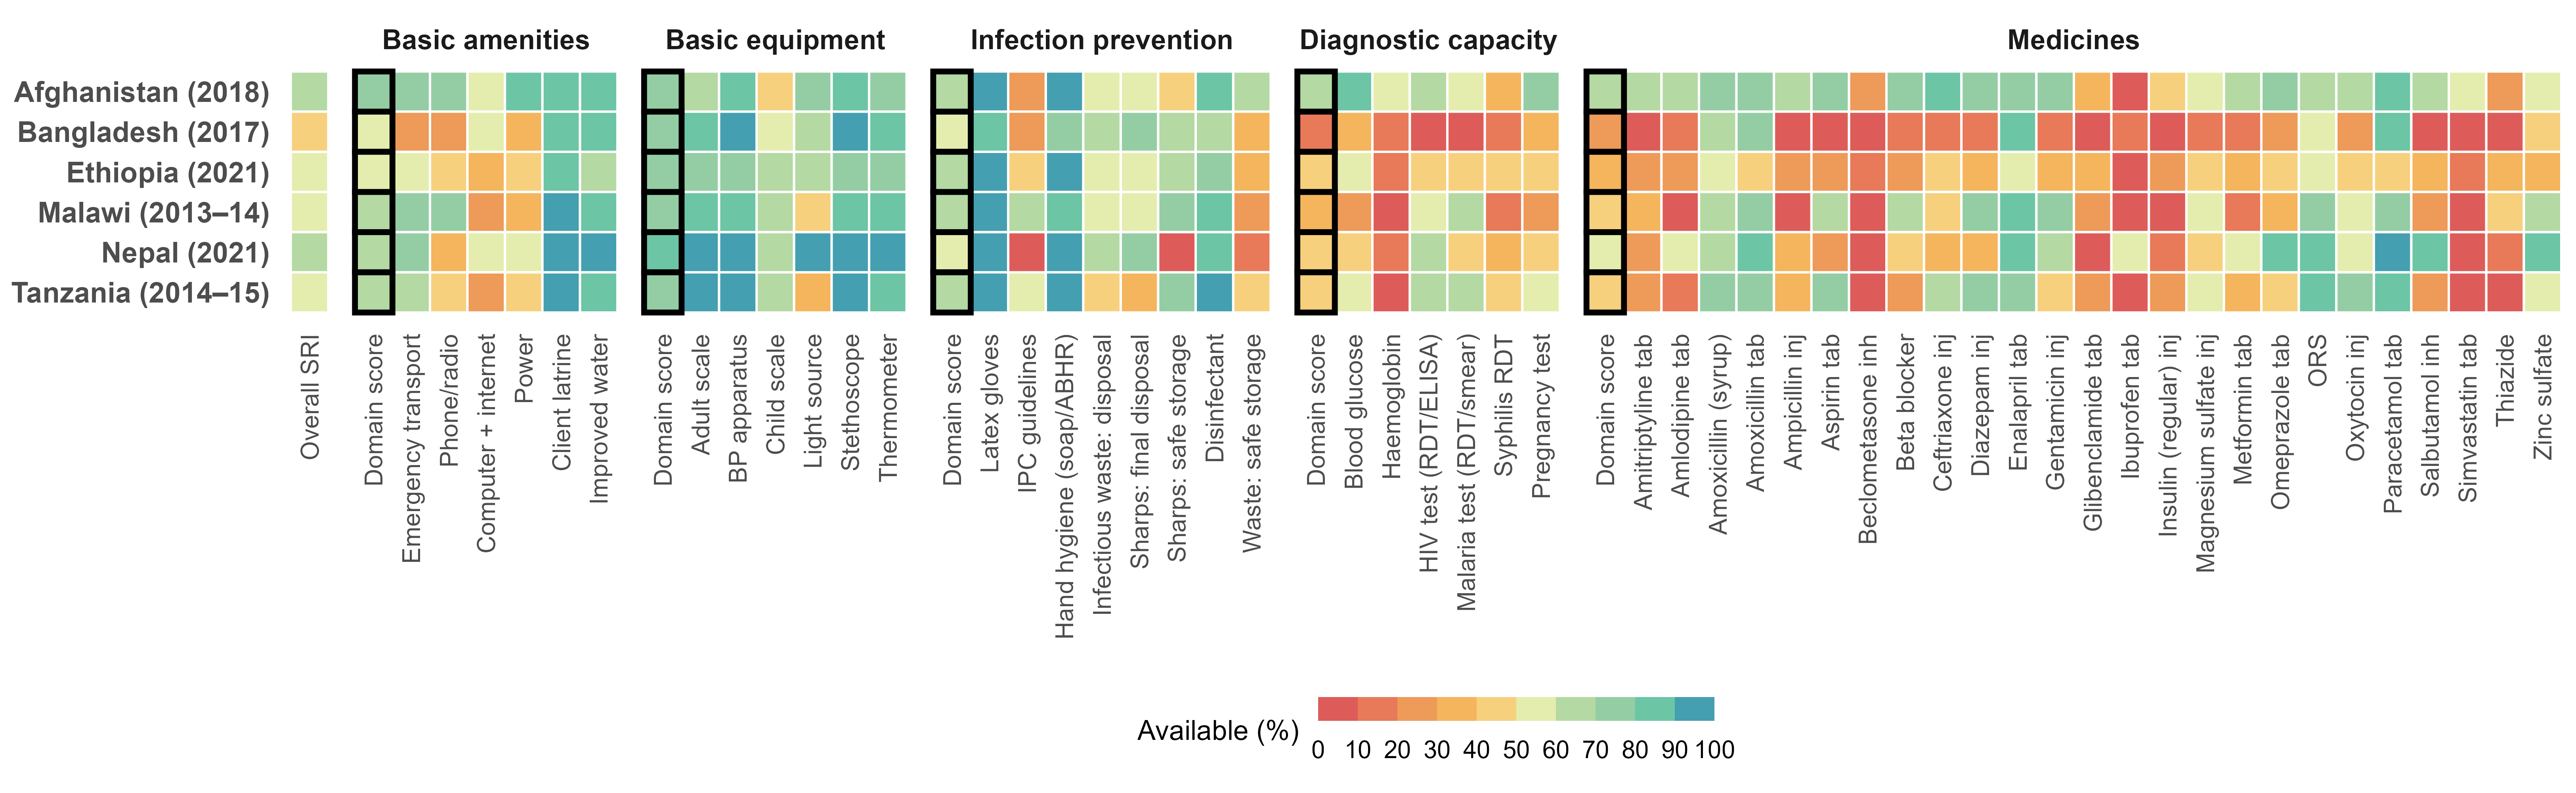
\includegraphics[width=9in]{images/figure1_sri_heatmap.png}
  \caption[Cross-country Service Readiness Index (SRI) profiles by domain and selected tracer items]{Cross-country Service Readiness Index (SRI) profiles by domain and selected tracer items. Domain scores are rescaled from 0--10 to 0--100; tracer items show the percentage of facilities with the item observed on the day of assessment. Higher values indicate greater readiness or item availability (see color bar).}
  \label{ch3:fig:sri_heatmap}
\end{figure}
\end{landscape}

 Vestibulum lacinia imperdiet massa. Praesent non massa blandit, bibendum dui eu, sodales arcu. Vestibulum scelerisque metus non tincidunt viverra. Orci varius natoque penatibus et magnis dis parturient montes, nascetur ridiculus mus. Morbi lacinia pretium arcu ut tincidunt. Etiam orci massa, efficitur id vehicula in, tincidunt ut eros. Vestibulum nec nulla vel metus varius efficitur in sit amet ipsum. Vestibulum rutrum elementum ullamcorper. Curabitur elit dui, interdum eu nibh id, congue suscipit lacus. Aenean velit lectus, mattis in odio ut, viverra pharetra tortor. Donec dapibus, tellus quis dictum aliquam, elit lacus dapibus eros, non consequat nunc orci quis odio. Vivamus ultricies convallis eros, sit amet sagittis velit consequat a. Fusce quis tortor sit amet ante bibendum pellentesque dignissim et diam.

Etiam semper rutrum enim elementum laoreet. Proin tristique sem metus, id sodales ante vulputate ut. Ut bibendum pulvinar nisi vitae condimentum. Pellentesque leo magna, semper eu dapibus sit amet, hendrerit non sapien. Morbi posuere facilisis urna, eget posuere quam porta non. Nam ac lacus diam. Suspendisse at quam elit. Nullam sagittis leo eget est vehicula mattis. 

\section{Discussion}

 Etiam semper rutrum enim elementum laoreet. Proin tristique sem metus, id sodales ante vulputate ut. Ut bibendum pulvinar nisi vitae condimentum. Pellentesque leo magna, semper eu dapibus sit amet, hendrerit non sapien. Morbi posuere facilisis urna, eget posuere quam porta non. Nam ac lacus diam. Suspendisse at quam elit. Nullam sagittis leo eget est vehicula mattis.

Proin venenatis mattis convallis. Morbi cursus pulvinar lorem, vel fringilla nibh bibendum sit amet. Phasellus ut lacus bibendum mi facilisis sodales. Pellentesque ultricies risus vitae viverra hendrerit. Fusce lobortis, dolor vel fringilla lobortis, tellus nibh ultricies lectus, quis placerat quam est a elit. Phasellus at quam finibus neque condimentum euismod sit amet nec est. Sed nec mollis nibh, a dapibus justo. Sed turpis lectus, lacinia quis sapien non, suscipit venenatis diam. Nunc facilisis ut arcu eu gravida. Sed felis sem, semper in sodales a, sodales a lacus. Sed lacinia nec nunc a ornare. Donec id nulla metus. Praesent viverra egestas justo, quis elementum dui posuere ac. Sed a condimentum velit, sit amet egestas eros. Nam iaculis, odio vel pharetra placerat, diam justo molestie sapien, sit amet fringilla massa magna id erat.

Nunc viverra rhoncus nulla, pretium interdum erat scelerisque quis. Cras ornare, libero et bibendum semper, quam elit accumsan tortor, sed efficitur libero ipsum non velit. Donec at justo suscipit, viverra arcu vestibulum, volutpat enim. Integer sed dapibus nunc. Nulla interdum nisl ligula, quis facilisis justo vestibulum et. Cras consequat egestas fringilla. Vestibulum nec commodo arcu, sit amet condimentum neque. Maecenas sed magna posuere, dignissim quam sit amet, euismod enim. Vivamus semper viverra turpis, eget viverra felis. Integer gravida molestie ex. Nam maximus et dolor a luctus. Integer bibendum, ante eu pellentesque pharetra, nibh ex condimentum ex, vitae eleifend dui lectus nec magna.







\clearpage
\input{ch4-example3}


%%% conclusions %%%%%%%%%%%%%%%%%%%%%%%%%%%%%%%%%%%%%%%%%%%%%%%%%%%%%%%%
\graphicspath{}
\chapter{Conclusion}

\noindent Some final thoughts here. Lorem ipsum dolor sit amet, consectetur adipiscing elit. Nullam non nunc libero. In sollicitudin luctus dapibus. Suspendisse potenti. Proin feugiat nisl et elit rutrum iaculis. Donec vel massa tempus, placerat justo in, ullamcorper mi. Nullam vel pellentesque augue. Vivamus iaculis turpis a arcu viverra, non rutrum nunc varius. Phasellus dignissim ante feugiat placerat tincidunt. Maecenas ut nulla sit amet lacus volutpat consequat et sed mauris. Praesent justo urna, aliquet quis aliquam in, tempor eu nunc. 

\section{Summary and synthesis of findings}

 Praesent eu aliquet orci, at pretium mauris. Proin ornare nibh sem, nec malesuada diam hendrerit quis. Nullam eu risus neque. Integer ultrices sit amet mi quis faucibus. Nulla sit amet libero ante. Nulla feugiat metus felis. Vivamus pulvinar finibus ornare. Aenean vulputate tincidunt mi vitae laoreet. Nam malesuada tristique quam, vitae tincidunt est tempor ut. Vestibulum vestibulum enim quis diam pellentesque, at tempor sapien pharetra. Ut felis libero, hendrerit eu accumsan vel, placerat ac sem. Proin facilisis blandit felis, id dignissim leo aliquam vel.

Vestibulum consectetur at mi vitae vestibulum. Proin tristique ultrices sollicitudin. Integer tortor lacus, luctus id rhoncus non, viverra tristique est. Maecenas scelerisque, nibh sit amet consectetur mollis, diam quam venenatis neque, eget accumsan mauris arcu sit amet quam. Donec eu orci nunc. Suspendisse et massa at dui eleifend tincidunt. Duis at faucibus orci. Morbi volutpat, odio eget facilisis mattis, tortor felis laoreet dui, eget euismod nibh nibh sed felis. Sed eget ullamcorper mauris. Quisque congue augue nec tempus luctus. Ut tempor lacus tortor, non hendrerit ante scelerisque a. Vivamus et elit faucibus, dapibus ex vel, ultricies nulla. Suspendisse nec odio malesuada, condimentum metus eu, venenatis ipsum. Sed magna lorem, porta nec leo ut, luctus maximus erat. 

\section{Contributions}

\subsection{Methodological contributions}

Suspendisse fermentum erat elit, ut egestas augue tempor in. Vivamus scelerisque, enim eget congue egestas, sem est ultricies felis, ac interdum felis velit sed quam. Quisque hendrerit egestas porttitor. Pellentesque habitant morbi tristique senectus et netus et malesuada fames ac turpis egestas. Quisque pretium dapibus diam vel cursus. Nulla faucibus pulvinar ligula, vitae vehicula velit mollis a. Donec justo ex, malesuada at dictum ut, lacinia eu nisl. Phasellus nisl orci, euismod vitae sagittis in, pretium ut tortor. Lorem ipsum dolor sit amet, consectetur adipiscing elit. Sed eu enim dignissim, viverra ligula at, porta lectus. Duis ac elit sit amet nisi commodo feugiat. Mauris sed tellus enim. 

\subsection{Substantive contributions}

 Vestibulum lacinia imperdiet massa. Praesent non massa blandit, bibendum dui eu, sodales arcu. Vestibulum scelerisque metus non tincidunt viverra. Orci varius natoque penatibus et magnis dis parturient montes, nascetur ridiculus mus. Morbi lacinia pretium arcu ut tincidunt. Etiam orci massa, efficitur id vehicula in, tincidunt ut eros. Vestibulum nec nulla vel metus varius efficitur in sit amet ipsum. Vestibulum rutrum elementum ullamcorper. Curabitur elit dui, interdum eu nibh id, congue suscipit lacus. Aenean velit lectus, mattis in odio ut, viverra pharetra tortor. Donec dapibus, tellus quis dictum aliquam, elit lacus dapibus eros, non consequat nunc orci quis odio. Vivamus ultricies convallis eros, sit amet sagittis velit consequat a. Fusce quis tortor sit amet ante bibendum pellentesque dignissim et diam. 

\section{Implications}

Etiam semper rutrum enim elementum laoreet. Proin tristique sem metus, id sodales ante vulputate ut. Ut bibendum pulvinar nisi vitae condimentum. Pellentesque leo magna, semper eu dapibus sit amet, hendrerit non sapien. Morbi posuere facilisis urna, eget posuere quam porta non. Nam ac lacus diam. Suspendisse at quam elit. Nullam sagittis leo eget est vehicula mattis.

Proin venenatis mattis convallis. Morbi cursus pulvinar lorem, vel fringilla nibh bibendum sit amet. Phasellus ut lacus bibendum mi facilisis sodales. Pellentesque ultricies risus vitae viverra hendrerit. Fusce lobortis, dolor vel fringilla lobortis, tellus nibh ultricies lectus, quis placerat quam est a elit. Phasellus at quam finibus neque condimentum euismod sit amet nec est. Sed nec mollis nibh, a dapibus justo. Sed turpis lectus, lacinia quis sapien non, suscipit venenatis diam. Nunc facilisis ut arcu eu gravida. Sed felis sem, semper in sodales a, sodales a lacus. Sed lacinia nec nunc a ornare. Donec id nulla metus. Praesent viverra egestas justo, quis elementum dui posuere ac. Sed a condimentum velit, sit amet egestas eros. Nam iaculis, odio vel pharetra placerat, diam justo molestie sapien, sit amet fringilla massa magna id erat. 

\section{Limitations}

Nunc viverra rhoncus nulla, pretium interdum erat scelerisque quis. Cras ornare, libero et bibendum semper, quam elit accumsan tortor, sed efficitur libero ipsum non velit. Donec at justo suscipit, viverra arcu vestibulum, volutpat enim. Integer sed dapibus nunc. Nulla interdum nisl ligula, quis facilisis justo vestibulum et. Cras consequat egestas fringilla. Vestibulum nec commodo arcu, sit amet condimentum neque. Maecenas sed magna posuere, dignissim quam sit amet, euismod enim. Vivamus semper viverra turpis, eget viverra felis. Integer gravida molestie ex. Nam maximus et dolor a luctus. Integer bibendum, ante eu pellentesque pharetra, nibh ex condimentum ex, vitae eleifend dui lectus nec magna. Nulla sagittis faucibus eros ut tincidunt. Aenean commodo accumsan est, eget elementum nibh malesuada eget. Praesent tempor quam non lacus malesuada, ac sollicitudin enim sodales. Proin at enim elementum magna vulputate semper. 

\section{Future work}



In rhoncus, ante ornare laoreet dictum, nunc diam laoreet risus, sed elementum lacus tellus nec sapien. Integer malesuada ante at turpis pulvinar feugiat. Aenean fermentum tincidunt molestie. Integer pharetra mattis tortor vel auctor. Aenean finibus a felis sit amet rhoncus. Phasellus non lectus et enim aliquet fermentum et ut nunc. Curabitur tincidunt placerat gravida.

Sed molestie augue non laoreet tempus. Nulla sagittis lectus vitae enim congue, ac aliquet mi fringilla. Vivamus quis lobortis metus. Phasellus iaculis nibh augue, in molestie leo malesuada eu. Etiam ultricies elit est, sed commodo massa suscipit vitae. Fusce pellentesque sit amet neque blandit interdum. Nullam purus ipsum, vulputate et pharetra ut, rhoncus nec ante. Fusce risus lacus, hendrerit eu felis eu, suscipit mollis lorem. Morbi nec urna eu metus elementum tempor quis ut mi. Vivamus venenatis varius enim, eu volutpat tellus suscipit nec. Mauris vulputate sit amet diam et condimentum. Fusce eget volutpat elit. 

\section{Final reflections}

 Cras ultricies sollicitudin lorem quis sodales. Aliquam ut leo eleifend, tristique purus eget, mollis nisi. Donec id libero in leo viverra varius nec ac enim. Sed tincidunt non lectus sed consequat. In eu mollis ipsum. Aenean placerat dolor in mi rhoncus varius. Donec dignissim ipsum sit amet enim auctor lobortis. Aliquam et nibh vel eros ultrices commodo sed at magna. Maecenas aliquet ante nec tempus lobortis.

Pellentesque sed risus eu lectus ultricies pharetra. Sed ac justo fringilla, volutpat elit sed, consequat nunc. Interdum et malesuada fames ac ante ipsum primis in faucibus. Mauris dignissim in purus nec lacinia. Pellentesque congue aliquam molestie. Sed id ultricies tellus. Mauris et mi dignissim, egestas tellus eu, pulvinar tortor. Pellentesque habitant morbi tristique senectus et netus et malesuada fames ac turpis egestas. Sed placerat nibh massa, ut volutpat dolor viverra et. Aenean non turpis eget lectus facilisis congue. Fusce lectus tortor, eleifend eget urna ornare, consequat tincidunt dui. 

%%% bibliography %%%%%%%%%%%%%%%%%%%%%%%%%%%%%%%%%%%%%%%%%%%%%%%%%%%%%%%
%
%  \printbibliography in biblatex is great, but doesn't allow for the
%  greatest customization, so we'll use the package biblatex + biber
%  backend to meet some requirements:
%
%  * bibliography should be an un-numbered chapter, and still have a
%    pdfbookmark and a line in the table of contents
%
%  * bibliography contents should be singlespace, and optionally a smaller
%    font
%
%  * first line of this "chapter" should be in the same spot as the first
%    line of preface sections (e.g., acknowledgement)
%
%  * we use \raggedright so things like URLs and DOIs aren't stretched out.
%
\clearpage
\chapter*{References}
\addcontentsline{toc}{chapter}{References}

\begin{singlespace}
  % Prevent entry splits across pages as much as possible
  \patchcmd{\bibsetup}{\interlinepenalty=5000}{\interlinepenalty=10000}{}{}

  % Single-space within entries, blank line between entries
  \setlength{\bibitemsep}{\baselineskip}

  % PHP/USC prefer clean ragged-right references
  \raggedright

  % Hanging indent for runovers
  \setlength{\bibhang}{0.5in}

  \printbibliography[heading=none]
  
\end{singlespace}


\newpage
\appendix

% Reset the chapter counter to represent A, B, C...
% \renewcommand{\thechapter}{\Alph{chapter}}

% \input{appx/ch1_supplement}
% \input{appx/ch2_supplement}
% \input{appx/ch3_appendices}
\chapter{Appendix Example and Some Guidance}
\label{appx:methods}

\doublespacing
\noindent Note that appendices still use double-spacing for text. Additionally, to comply with the formatting guidance that appendices should not use table / figure numbering and should instead reference only the appendix itself, you can use the * to remove prevent number. For example \texttt{\textbackslash caption*\{DHS displacement procedure visualization\}}.

You can include multiple appendix files, but in this example, I have included only one.

\begin{itemize}
    \item \textbf{Step 1:} A random angle is drawn
    \item \textbf{Step 2:} Random distance (between 0 km and 2 km in urban areas, between 0 km and 5 km in rural, with 1\% of rural clusters displaced between 0 and 10 km)
    \item \textbf{Step 3:} If displaced location falls outside of admin boundary (the district level in Malawi), the steps 1 and 2 are repeated.
\end{itemize}

\begin{figure}[H]
  \centering
    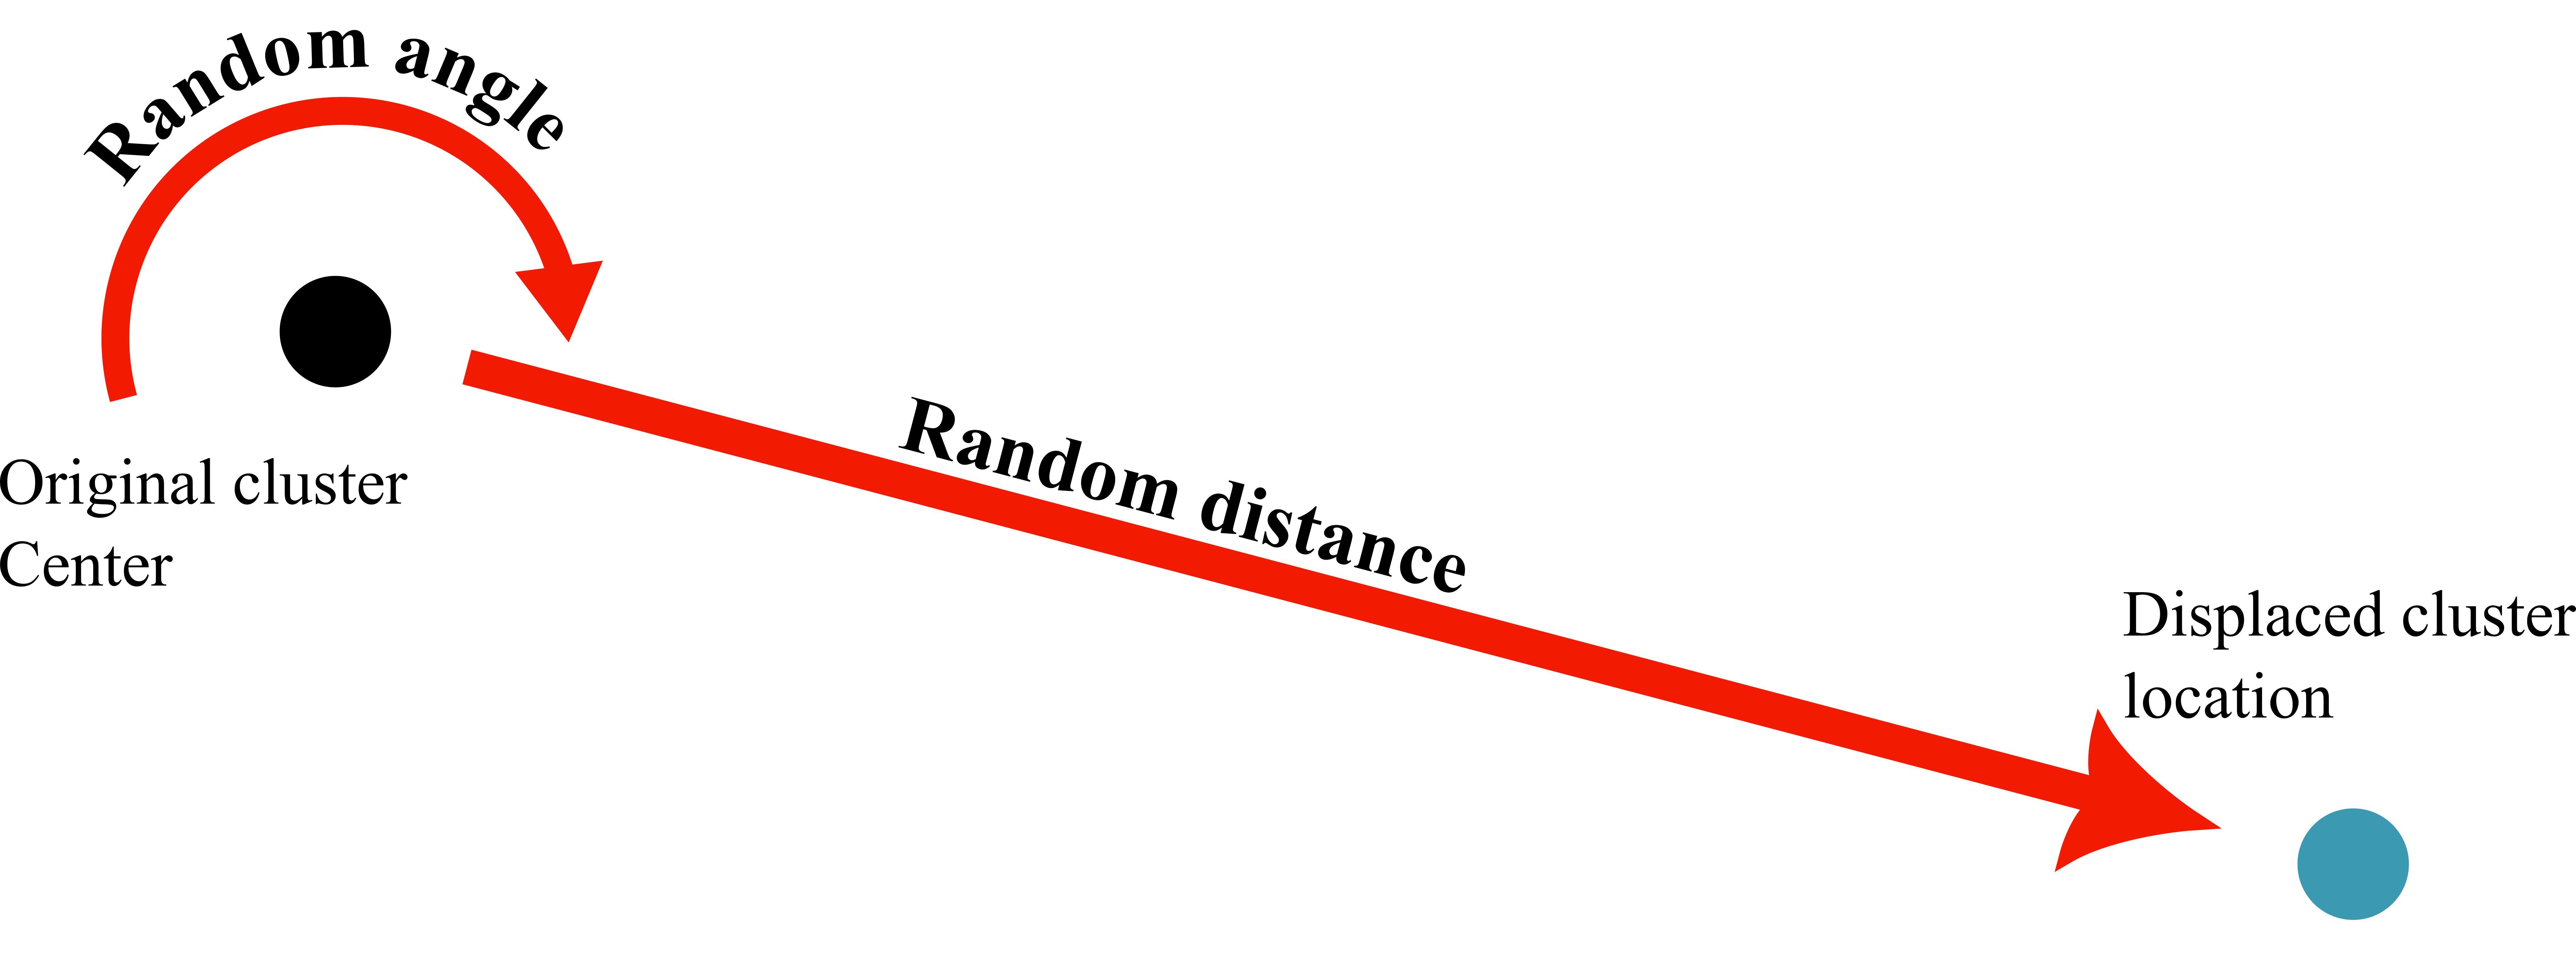
\includegraphics[width=6in]{images/displacement.png}
  % 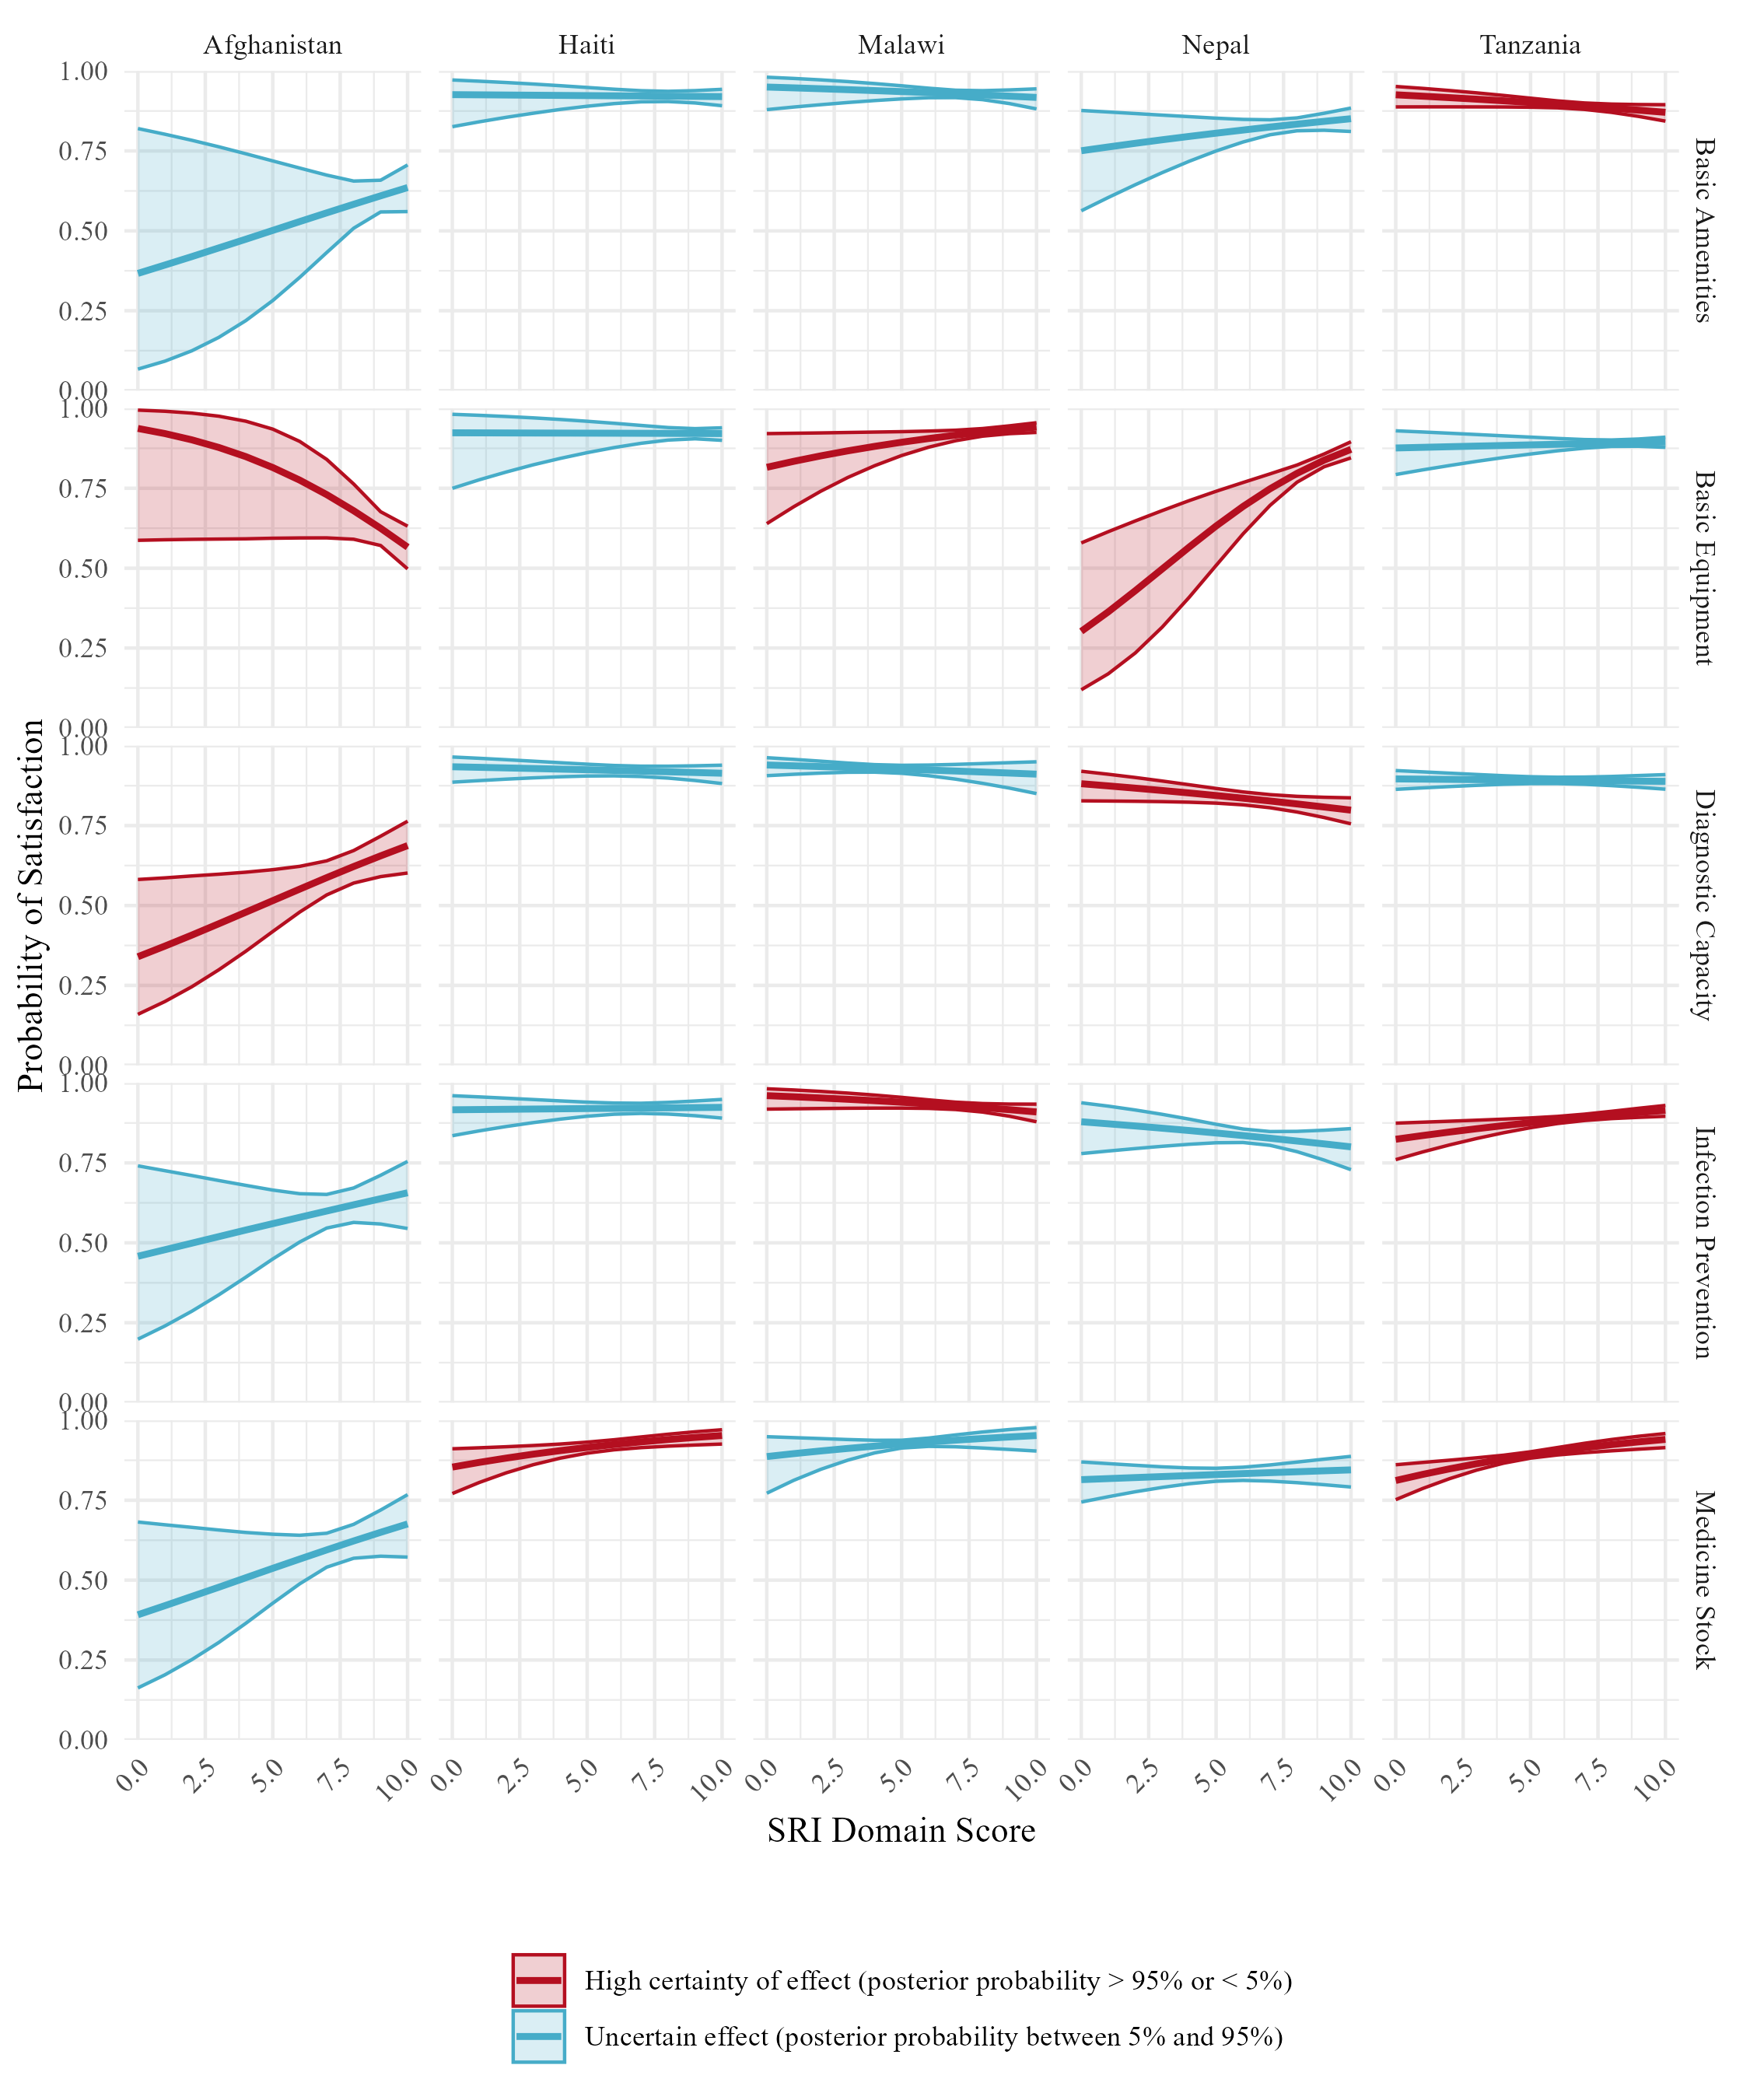
\includegraphics[width=7.5in, height=9in]{images/an_marginalEffects.png}
  \caption*{DHS displacement procedure visualization}
  \label{fig-displacement}
\end{figure}

Proin venenatis mattis convallis. Morbi cursus pulvinar lorem, vel fringilla nibh bibendum sit amet. Phasellus ut lacus bibendum mi facilisis sodales. Pellentesque ultricies risus vitae viverra hendrerit. Fusce lobortis, dolor vel fringilla lobortis, tellus nibh ultricies lectus, quis placerat quam est a elit. Phasellus at quam finibus neque condimentum euismod sit amet nec est. Sed nec mollis nibh, a dapibus justo. Sed turpis lectus, lacinia quis sapien non, suscipit venenatis diam. Nunc facilisis ut arcu eu gravida. Sed felis sem, semper in sodales a, sodales a lacus. Sed lacinia nec nunc a ornare. Donec id nulla metus. Praesent viverra egestas justo, quis elementum dui posuere ac. Sed a condimentum velit, sit amet egestas eros. Nam iaculis, odio vel pharetra placerat, diam justo molestie sapien, sit amet fringilla massa magna id erat. 

% \[
% f_j(s)=
% \begin{cases}
% \dfrac{1}{2\pi r_j d(s,\tilde{s}_j)}, & d(s,\tilde{s}_j)\le r_j,\\[6pt]
% 0, & \text{otherwise},
% \end{cases}
% \]
    \begin{equation}
    \label{eq:pdf}
f_j(x_{0},y_{0}) = 
\begin{dcases}
\frac{1}{2\pi r_j\sqrt{x_{0}^{2}+y_{0}^{2}}}, & \text{if } 0 < \sqrt{x_{0}^2 + y_{0}^2} \leq r_j \\
0, & \text{otherwise.}
\end{dcases}
\end{equation}

\noindent where $x_0$ and $y_0$ denote projected coordinate offsets from the released cluster location $\tilde{s}_j$, and the singularity at $\sqrt{x_0^2+y_0^2}=0$ can be ignored in practice by excluding the zero-distance point from integral calculations.

Nam maximus et dolor a luctus. Integer bibendum, ante eu pellentesque pharetra, nibh ex condimentum ex, vitae eleifend dui lectus nec magna. Nulla sagittis faucibus eros ut tincidunt. Aenean commodo accumsan est, eget elementum nibh malesuada eget. Praesent tempor quam non lacus malesuada, ac sollicitudin enim sodales. Proin at enim elementum magna vulputate semper. 


\begin{figure}[H]
  \centering
    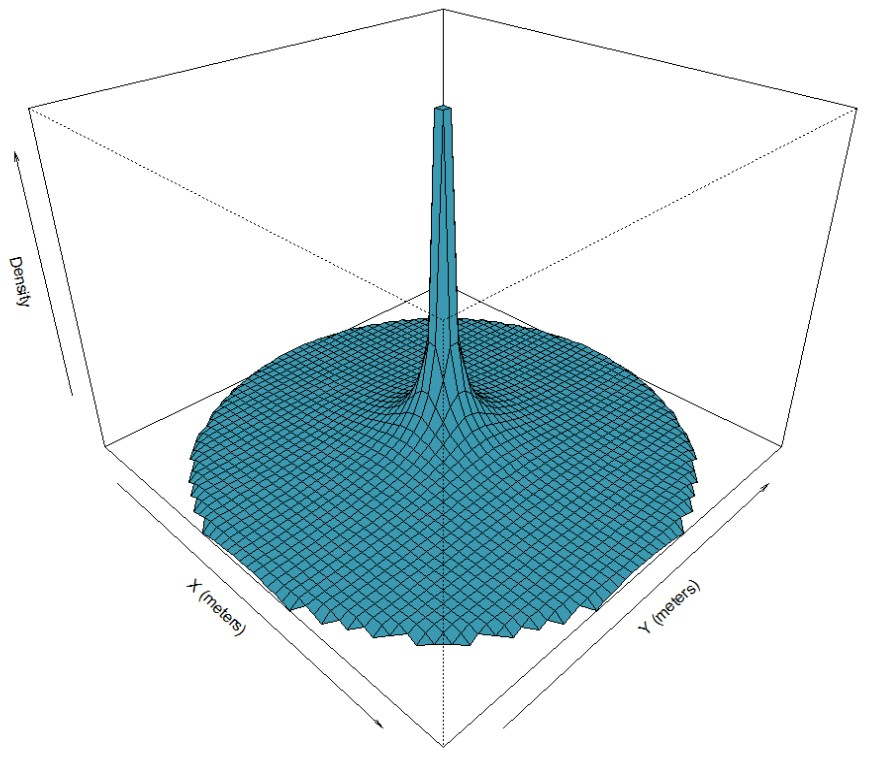
\includegraphics[height=4in]{images/DensityPlot.jpg}
  % 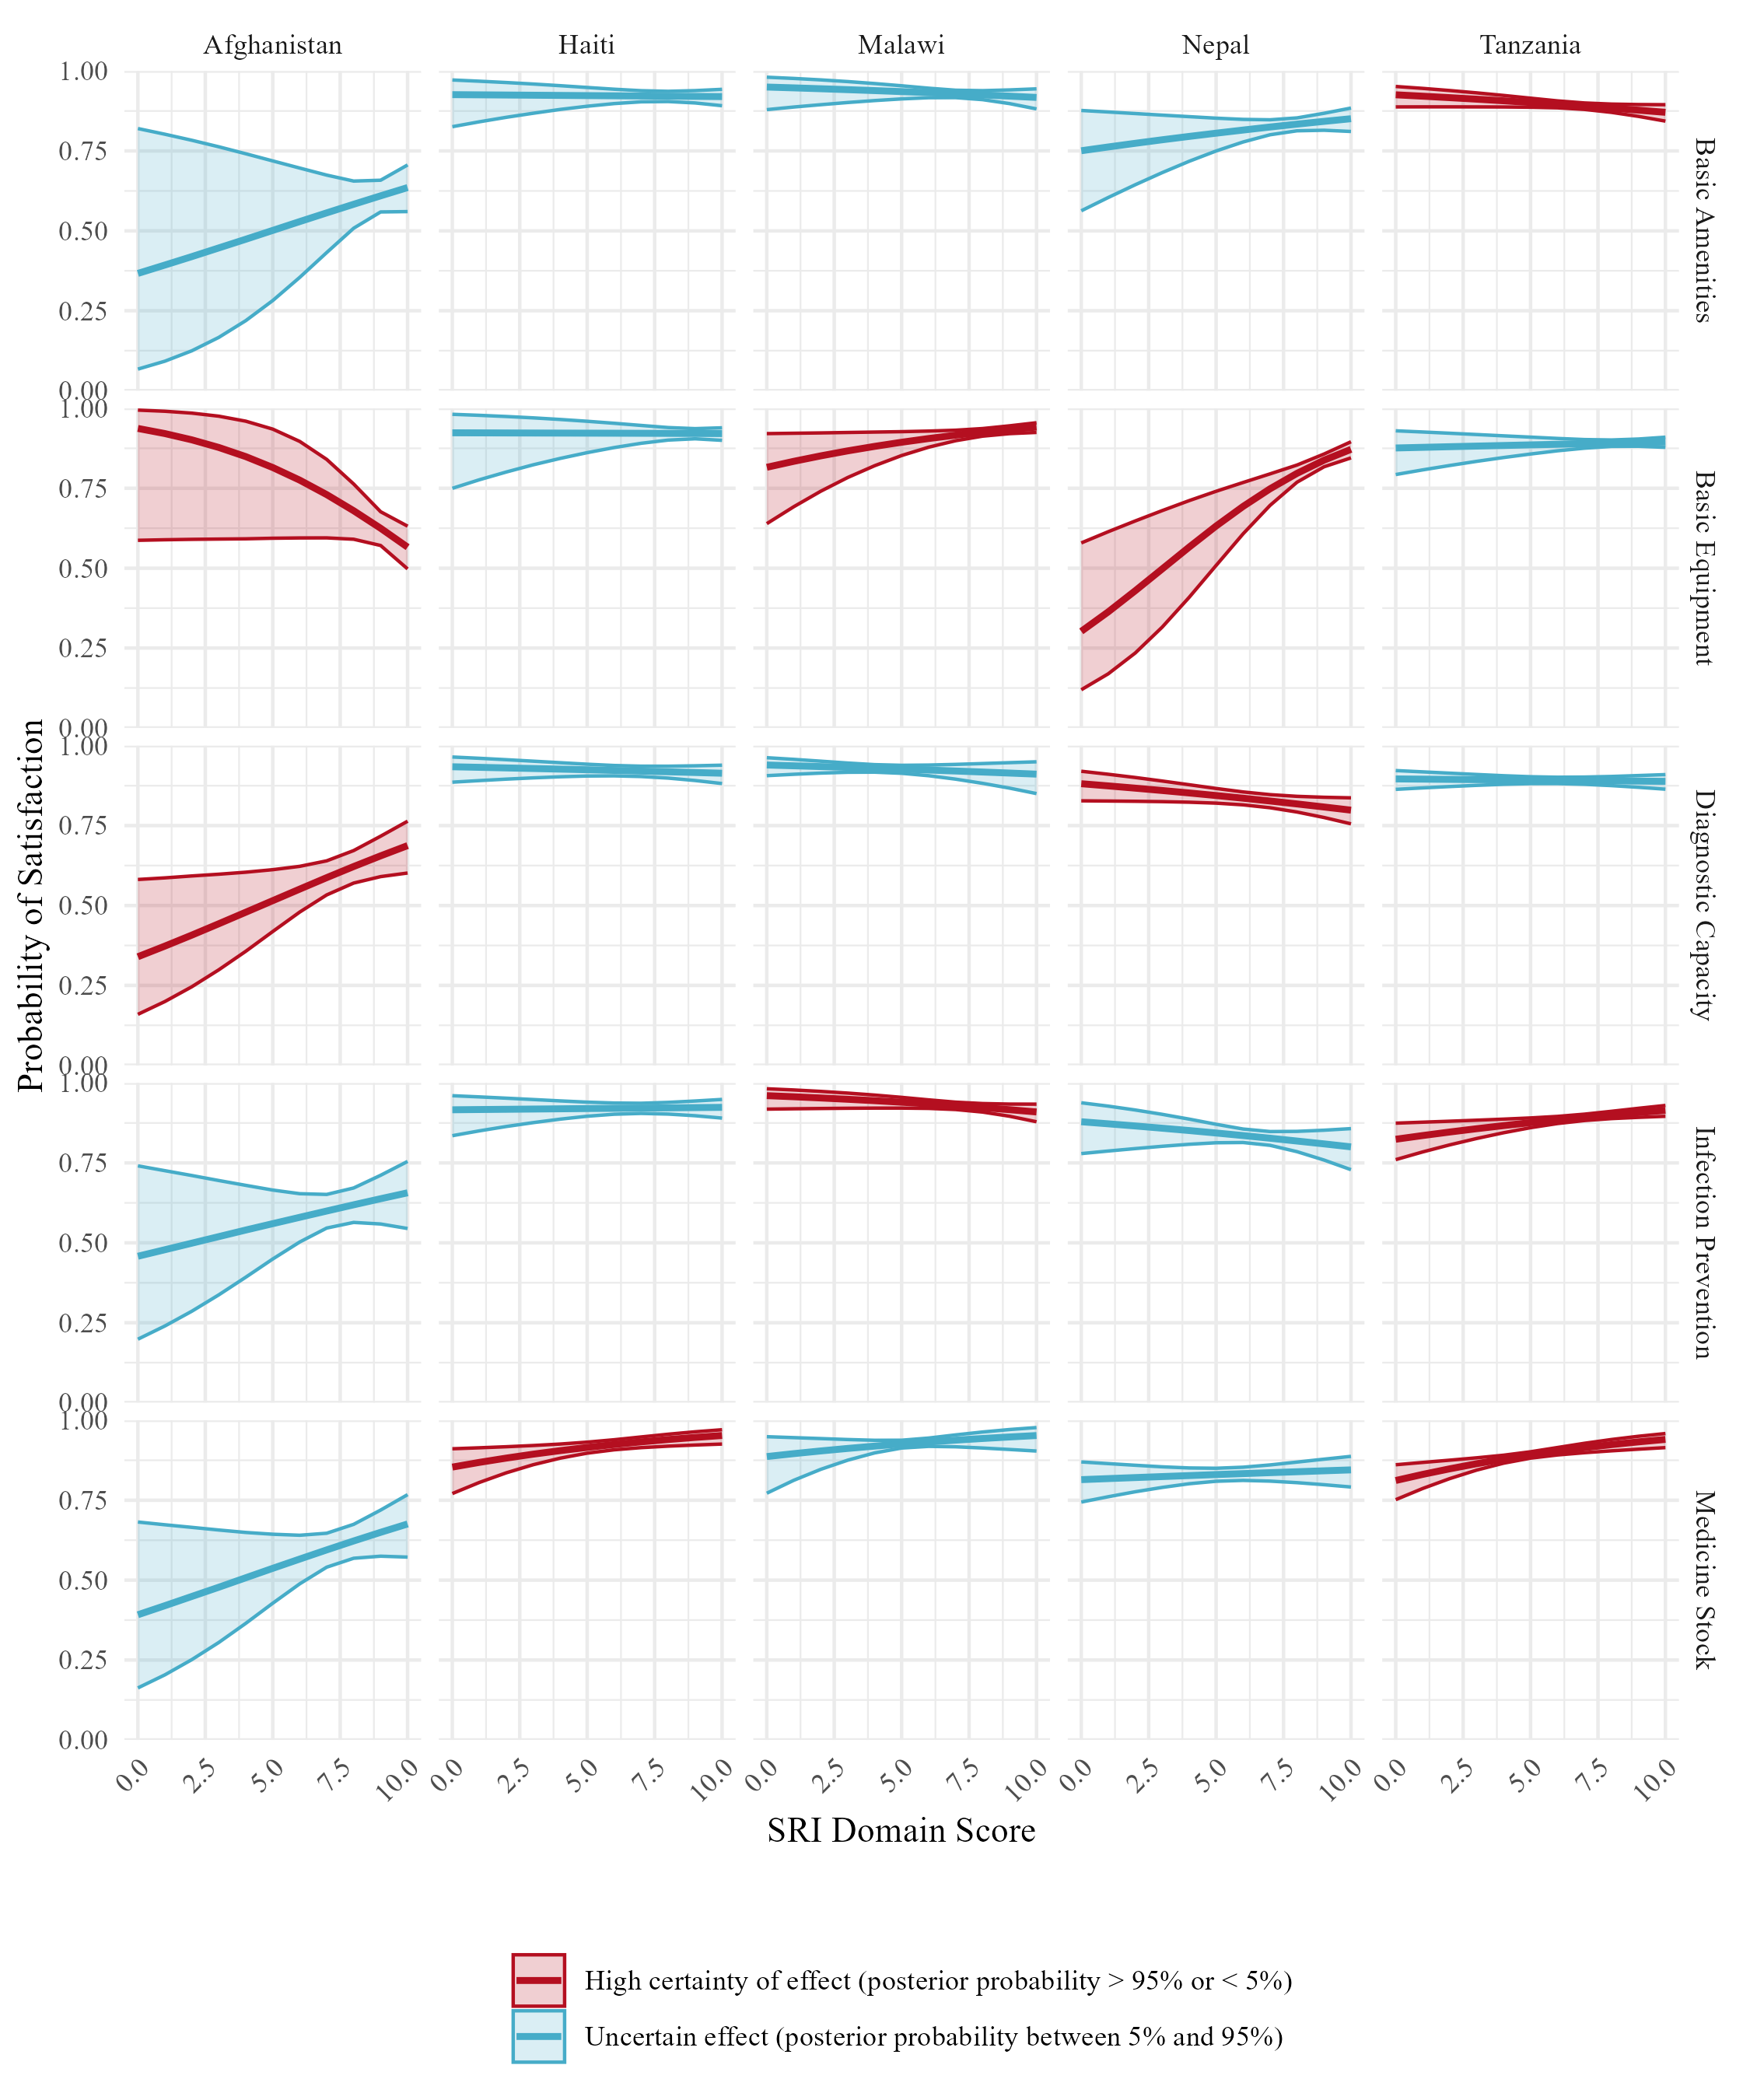
\includegraphics[width=7.5in, height=9in]{images/an_marginalEffects.png}
  \caption*{Visualization of the surface created by the equation above}
  \label{fig-pdf_plot}
\end{figure}

 Nunc viverra rhoncus nulla, pretium interdum erat scelerisque quis. Cras ornare, libero et bibendum semper, quam elit accumsan tortor, sed efficitur libero ipsum non velit. Donec at justo suscipit, viverra arcu vestibulum, volutpat enim. Integer sed dapibus nunc. Nulla interdum nisl ligula, quis facilisis justo vestibulum et. Cras consequat egestas fringilla. Vestibulum nec commodo arcu, sit amet condimentum neque. Maecenas sed magna posuere, dignissim quam sit amet, euismod enim. Vivamus semper viverra turpis, eget viverra felis. Integer gravida molestie ex. Nam maximus et dolor a luctus. Integer bibendum, ante eu pellentesque pharetra, nibh ex condimentum ex, vitae eleifend dui lectus nec magna.



\chapter{Sensitivity tests using half-Cauchy priors for the random intercept standard deviation}
\label{appx:half-cauchy}

\begin{table}[H]
\centering
\begin{threeparttable}

\singlespacing    
\caption*{Sensitivity analysis: Bayesian multilevel logistic regression models for antenatal care utilization, Malawi, using a half-Cauchy prior for the cluster-level random intercept standard deviation. Posterior median odds ratios (OR), 95\% credible intervals, and posterior probability of direction (PD).}
\label{tbl:app_anc_models_halfcauchy_mw}
{\fontsize{11pt}{13.2pt}\selectfont
\begin{tabular}{l ll ll}
\hline
\hline
 & \multicolumn{2}{c}{4+ ANC visits} & \multicolumn{2}{c}{ANC initiation (1st trimester)} \\
 & OR & PD$^{\dagger}$ & OR & PD$^{\dagger}$ \\
 & 95\% CrI &  & 95\% CrI &  \\
\hline

\textbf{Health service environment (cluster-level)} & & & & \\
\hspace{2pt} Essential medicines readiness (0--10) & 1.05 & 99.6\% & 1.05 & 99.0\% \\
 & (1.01 -- 1.08) & & (1.01 -- 1.10) & \\
\hspace{2pt} Service availability (days/month) & 1.00 & 74.1\% & 1.00 & 80.0\% \\
 & (0.99 -- 1.01) & & (0.99 -- 1.01) & \\
\hspace{2pt} Pr(nearest facility charges fees) (per 10pp)$^{\S}$ & 1.00 & 57.0\% & 0.98 & 100.0\% \\
 & (0.99 -- 1.01) & & (0.96 -- 0.99) & \\
\hspace{2pt} Distance to nearest facility (km) & 0.98 & 98.2\% & 0.99 & 84.1\% \\
 & (0.96 -- 1.00) & & (0.96 -- 1.01) & \\

\textbf{Individual and household characteristics} & & & & \\
\hspace{2pt} Rural residence & 0.95 & 75.4\% & 1.16 & 94.8\% \\
 & (0.81 -- 1.11) & & (0.97 -- 1.41) & \\
\hspace{2pt} Household wealth (quintile) & 1.03 & 97.9\% & 1.06 & 99.9\% \\
 & (1.00 -- 1.07) & & (1.02 -- 1.10) & \\
\hspace{2pt} Maternal age at index birth (years) & 1.03 & 100.0\% & 1.02 & 99.7\% \\
 & (1.02 -- 1.04) & & (1.00 -- 1.03) & \\
\hspace{2pt} Respondent education (years) & 1.03 & 100.0\% & 1.01 & 97.1\% \\
 & (1.01 -- 1.04) & & (1.00 -- 1.03) & \\
\hspace{2pt} Parity (birth order) & 0.94 & 100.0\% & 0.95 & 99.5\% \\
 & (0.91 -- 0.97) & & (0.92 -- 0.99) & \\

\hline
\textit{Random intercept SD (cluster)} & 0.40 & & 0.53 & \\
 & (0.34 -- 0.45) & & (0.47 -- 0.60) & \\
Observations & 13,448 & & 13,448 & \\
Clusters (DHSID) & 850 & & 850 & \\
\hline

% \multicolumn{5}{p{16cm}}{\footnotesize
% ORs are posterior medians from Bayesian multilevel logistic regression models with a cluster-level random intercept (DHSID). Cluster-level health service environment measures were constructed using a probabilistic linkage procedure accounting for DHS geographic displacement. Sensitivity models used a half-Cauchy prior for the cluster-level random intercept standard deviation (see Appendix \ref{appx:half-cauchy}). Credible intervals are equal-tailed (95\%). 
% $^{\dagger}$ The posterior probability of direction (PD) is the posterior probability that the estimated effect is strictly positive or strictly negative (whichever is larger), reflecting the strength of evidence for the direction of the association. 
% $^{\S}$ Fee exposure is scaled such that a one-unit increase corresponds to a 10 percentage-point increase in the probability that the nearest facility charges fees.}

\end{tabular}

\begin{tablenotes}[flushleft]
\fontsize{9pt}{10.5pt}\selectfont
\setlength{\itemsep}{0pt}
\setlength{\parsep}{0pt}
\setlength{\leftskip}{0pt}
\item ORs are posterior medians from Bayesian multilevel logistic regression models with a cluster-level random intercept (DHSID). Cluster-level health service environment measures were constructed using a probabilistic linkage procedure accounting for DHS geographic displacement. Sensitivity models used a half-Cauchy prior for the cluster-level random intercept standard deviation (see Appendix \ref{appx:half-cauchy}). Credible intervals are equal-tailed (95\%). 
$^{\dagger}$ The posterior probability of direction (PD) is the posterior probability that the estimated effect is strictly positive or strictly negative (whichever is larger), reflecting the strength of evidence for the direction of the association. 
$^{\S}$ Fee exposure is scaled such that a one-unit increase corresponds to a 10 percentage-point increase in the probability that the nearest facility charges fees.
\end{tablenotes}

}
\end{threeparttable}
\end{table}





\restoregeometry

% % Manually increment the chapter counter
% \stepcounter{chapter}

\end{document}
